\section{Experiments}
\label{sec:experiments}
We designed \methodname{} primarily for the zero-shot setting, where labels that are used for inference have never been seen during training. However, due to a lack of a standardized protocol and sufficient datasets and baselines for the zero-shot setting, we compare \methodname{} to zero- and few-shot semantic segmentation models on few-shot benchmarks. Note that few-shot methods have access to more information and are thus expected to yield higher accuracy. However, the need for labeled samples severely restricts their flexibility compared to our approach. 


\subsection{Experimental Setup}
We follow the protocol of the recent state-of-the-art few-shot method HSNet~\citep{min2021hypercorrelation} and evaluate on three widely-used few-shot semantic segmentation benchmarks: {PASCAL-5$^i$~\citep{Everingham15}}, COCO-20$^i$~\citep{lin2014microsoft}, and FSS-1000~\citep{li2020fss}. Following a standard protocol for few-shot segmentation, we use the mean intersection over union (mIoU) and foreground-background intersection of union (FB-IoU) as the evaluation metrics. The mIoU calculates the average IoU over all classes, FB-IoU computes mean value of foreground and background IoUs in fold $i$ and ignores the object classes. 

When not stated otherwise we use an \methodname{} model with the
text encoder provided by CLIP-ViT-B/32 and leverage DPT with a ViT-L/16 backbone as the image encoder. For datasets that provide a background or unknown class, we set the corresponding background label to ``other''. We use SGD with momentum 0.9 and a polynomial learning rate scheduler with decay rate 0.9. We train with a batch size of $6$ on six Quadro RTX 6000.

\begin{table}[t]
    \centering
    \resizebox{0.9\columnwidth}{!}{%
\begin{tabular}{c|c|c|cccccc}
\toprule 

Model&Backbone&Method& $5^0$ & $5^1$ & $5^2$ & $5^3$ &mean&FB-IoU \\  
\midrule\midrule
OSLSM&&1-shot&33.6&55.2&40.9&33.5& 40.8 & 61.3\\
co-FCN&VGG16&1-shot&36.7 &50.6& 44.9& 32.4& 41.1 & 60.1\\
AMP-2&&1-shot&41.9  &50.2 &46.7 &34.7 &43.4 & 61.9\\
\midrule
PANet&\multirow{2}{*}{ResNet50}&1-shot&44.0 &57.5& 50.8& 44.0 &49.1&- \\
PGNet&&1-shot&56.0& 66.9 &50.6& 50.4& 56.0& 69.9 \\
\midrule
FWB&\multirow{6}{*}{ResNet101}&1-shot&51.3 & 64.5 &56.7& 52.2& 56.2 &- \\
PPNet&&1-shot&52.7 &62.8 &57.4& 47.7& 55.2&  70.9\\
DAN&&1-shot&54.7& 68.6& 57.8& 51.6& 58.2& 71.9\\
PFENet&&1-shot&60.5& 69.4& 54.4& 55.9& 60.1& 72.9\\
RePRI&&1-shot&59.6& 68.6& \textbf{62.2}& 47.2& 59.4&  -\\
HSNet&&1-shot&\textbf{67.3} &\textbf{72.3} & 62.0 &\textbf{63.1}& \textbf{66.2}& \textbf{77.6} \\
\midrule
SPNet&\multirow{2}{*}{ResNet101}&zero-shot&23.8	&17.0&14.1&18.3&18.3&44.3\\
ZS3Net&&zero-shot&40.8&39.4&39.3&33.6&38.3&57.7\\
\midrule
\methodname{} &ResNet101&zero-shot&\textbf{52.8}&\textbf{53.8}&\textbf{44.4}&\textbf{38.5}&\textbf{47.4}&\textbf{64.1} \\

\methodname{} &ViT-L/16&zero-shot&\textbf{61.3}&\textbf{63.6}&\textbf{43.1}&\textbf{41.0}&\textbf{52.3}&\textbf{67.0} \\
\bottomrule
\end{tabular}
}
\caption{Comparison of mIoU and FB-IoU (higher is better) on PASCAL-$5^i$.}




    \label{tab:fewshot_pascal}
\end{table}

\begin{table}[t]
    \centering
    \begin{tabular}{c|c|c|cccccc}
\toprule 

Model&Backbone&Method& $20^0$ & $20^1$ & $20^2$ & $20^3$ &mean&FB-IoU \\  
\midrule\midrule
PPNet&\multirow{4}{*}{ResNet50}&1-shot&28.1& 30.8& 29.5 &27.7&  29.0 & - \\
PMM&&1-shot&29.3 &34.8& 27.1 &27.3&  29.6& -  \\
RPMM&&1-shot&29.5& 36.8& 28.9& 27.0&   30.6 &- \\
RePRI&&1-shot&32.0& 38.7& 32.7& 33.1 & 34.1 & - \\
\midrule
FWB&\multirow{4}{*}{ResNet101}&1-shot&17.0 &18.0 &21.0 &28.9&  21.2 &- \\
DAN&&1-shot&-&-&-&-&24.4& 62.3 \\
PFENet&&1-shot&36.8 & 41.8& 38.7& 36.7 &38.5 & 63.0 \\
HSNet&&1-shot&\textbf{37.2}& \textbf{44.1}& \textbf{42.4}& \textbf{41.3}&  \textbf{41.2}  &\textbf{69.1} \\
\midrule
ZS3Net&ResNet101&zero-shot&18.8&20.1&24.8&20.5&  21.1	&55.1 \\
\midrule
\methodname{} &ResNet101&zero-shot&\textbf{22.1}&\textbf{25.1}&\textbf{24.9}&\textbf{21.5}&\textbf{23.4}&\textbf{57.9} \\

\methodname{} &ViT-L/16&zero-shot&\textbf{28.1}&\textbf{27.5}&\textbf{30.0}&\textbf{23.2}&\textbf{27.2}  &\textbf{59.9} \\
\bottomrule
\end{tabular}
\caption{Comparison of mIoU and FB-IoU (higher is better) on COCO-$20^i$. }

    \label{tab:fewshot_coco}
    \vspace{-0.2in}
\end{table}

\subsection{PASCAL-5$^i$ and COCO-20$^i$}
PASCAL-5$^i$ and COCO-20$^i$ are few-shot segmentation datasets that have been created from PASCAL VOC 2012~\citep{Everingham15} and the COCO dataset~\citep{lin2014microsoft}, respectively. PASCAL-5$^i$ is composed of 20 object classes with corresponding mask annotations and has been evenly divided into 4 folds of 5 classes each. We denote different folds by 5$^i$, where $i \in \{0, 1, 2, 3\}$. Similarly, COCO-20$^i$ is composed of 4 folds of 20 classes each. 


 We compare \methodname{} to various state-of-the-art few-shot models: OSLSM~\citep{shaban2017one}, Co-FCN~\citep{rakelly2018conditional}, AMP-2~\citep{siam2019amp}, PANet~\citep{wang2019panet}, PGNet~\citep{zhang2019pyramid}, FWB~\citep{nguyen2019feature}, PPNet~\citep{liu2020part}, DAN~\citep{wang2020few}, PFENet~\citep{tian2020prior}, RePRI~\citep{boudiaf2021few}, and HSNet~\citep{min2021hypercorrelation}. These few-shot methods propose strategies to segment unseen objects based on pretraining on seen categories and finetuning with a few images from the  target class.
 In addition, we also compare to the competitive zero-shot baseline ZS3Net~\citep{bucher2019zero}, which adopts the DeepLabv3+ framework and to~\citet{xian2019semantic} which leverages DeepLabv2. We follow their official code, training setting and training steps on the basis of their provided model pretrained on ImageNet~\citep{deng2009imagenet}. We follow the common experimental setup~\citep{nguyen2019feature} 
 and conduct cross-validation over all folds. Assuming that $n_i$ is the number of classes in fold $i$, for each fold $i$, we use images of other folds for training and randomly sampled 1000 images of target fold $i$ for evaluation. We show PASCAL-5$^i$ and COCO-20$^i$ results in Tables~\ref{tab:fewshot_pascal} and~\ref{tab:fewshot_coco}. Our model (with the same ResNet101 backbone) outperforms the zero-shot baseline by a considerable margin across folds and datasets and is even competitive with several few-shot methods. We also observe an obvious edge of \methodname{} by using a larger backbone (ViT-L/16).
 \begin{wraptable}{R}{0.5\linewidth} %[t]
%\vspace{-0.4in}
    \centering
    \scalebox{0.8}{
\begin{tabular}{c|c|c|c}
\toprule 
Model&Backbone& Method&mIoU \\  
\midrule\midrule
OSLSM & \multirow{4}{*}{VGG16} &1-shot&70.3\\
GNet&&1-shot&71.9\\
FSS&&1-shot&73.5\\
DoG-LSTM&&1-shot&80.8\\
\midrule
DAN&\multirow{2}{*}{ResNet101}&1-shot&85.2\\
HSNet&&1-shot&86.5 \\
\midrule
\methodname{} &ResNet101&zero-shot&84.7 \\
\methodname{} &ViT-L/16&zero-shot&\textbf{87.8} \\
\bottomrule
\end{tabular}
}
\caption{Comparison of mIoU on FSS-1000.}



    \label{tab:fewshot_fss}
\end{wraptable}

%\vspace{-0.1in}
\subsection{FSS-1000}
FSS-1000~\citep{li2020fss} is a recent benchmark dataset for few-shot segmentation. It consists of 1000 object classes with pixelwise annotated segmentation masks. It contains a significant number of unseen or unannotated objects in comparison to previous datasets such as PASCAL and COCO. Following the standard protocol, we split the 1000 classes into training, validation, and test classes, with 520, 240, and 240 classes, respectively. We use a base learning rate of 0.05 and train the model for 60 epochs. 

Table~\ref{tab:fewshot_fss} compares our approach to state-of-the-art few-shot models. Notably, under the same ResNet101, \methodname{} could achieve comparative results of the state-of-the-art one-shot method. Also, \methodname{} even outperforms a state-of-the-art one-shot method: 87.8 mIoU (ours) vs. 86.5 mIoU (HSNet) with a larger backbone ViT-L/16, indicating that \methodname{} generalizes very well to unseen categories. Figure~\ref{fig:example_illustration1} shows examples of segmentation results on unseen categories.

 \begin{figure}[htb!]
    \centering
    \vspace{0.1in}
     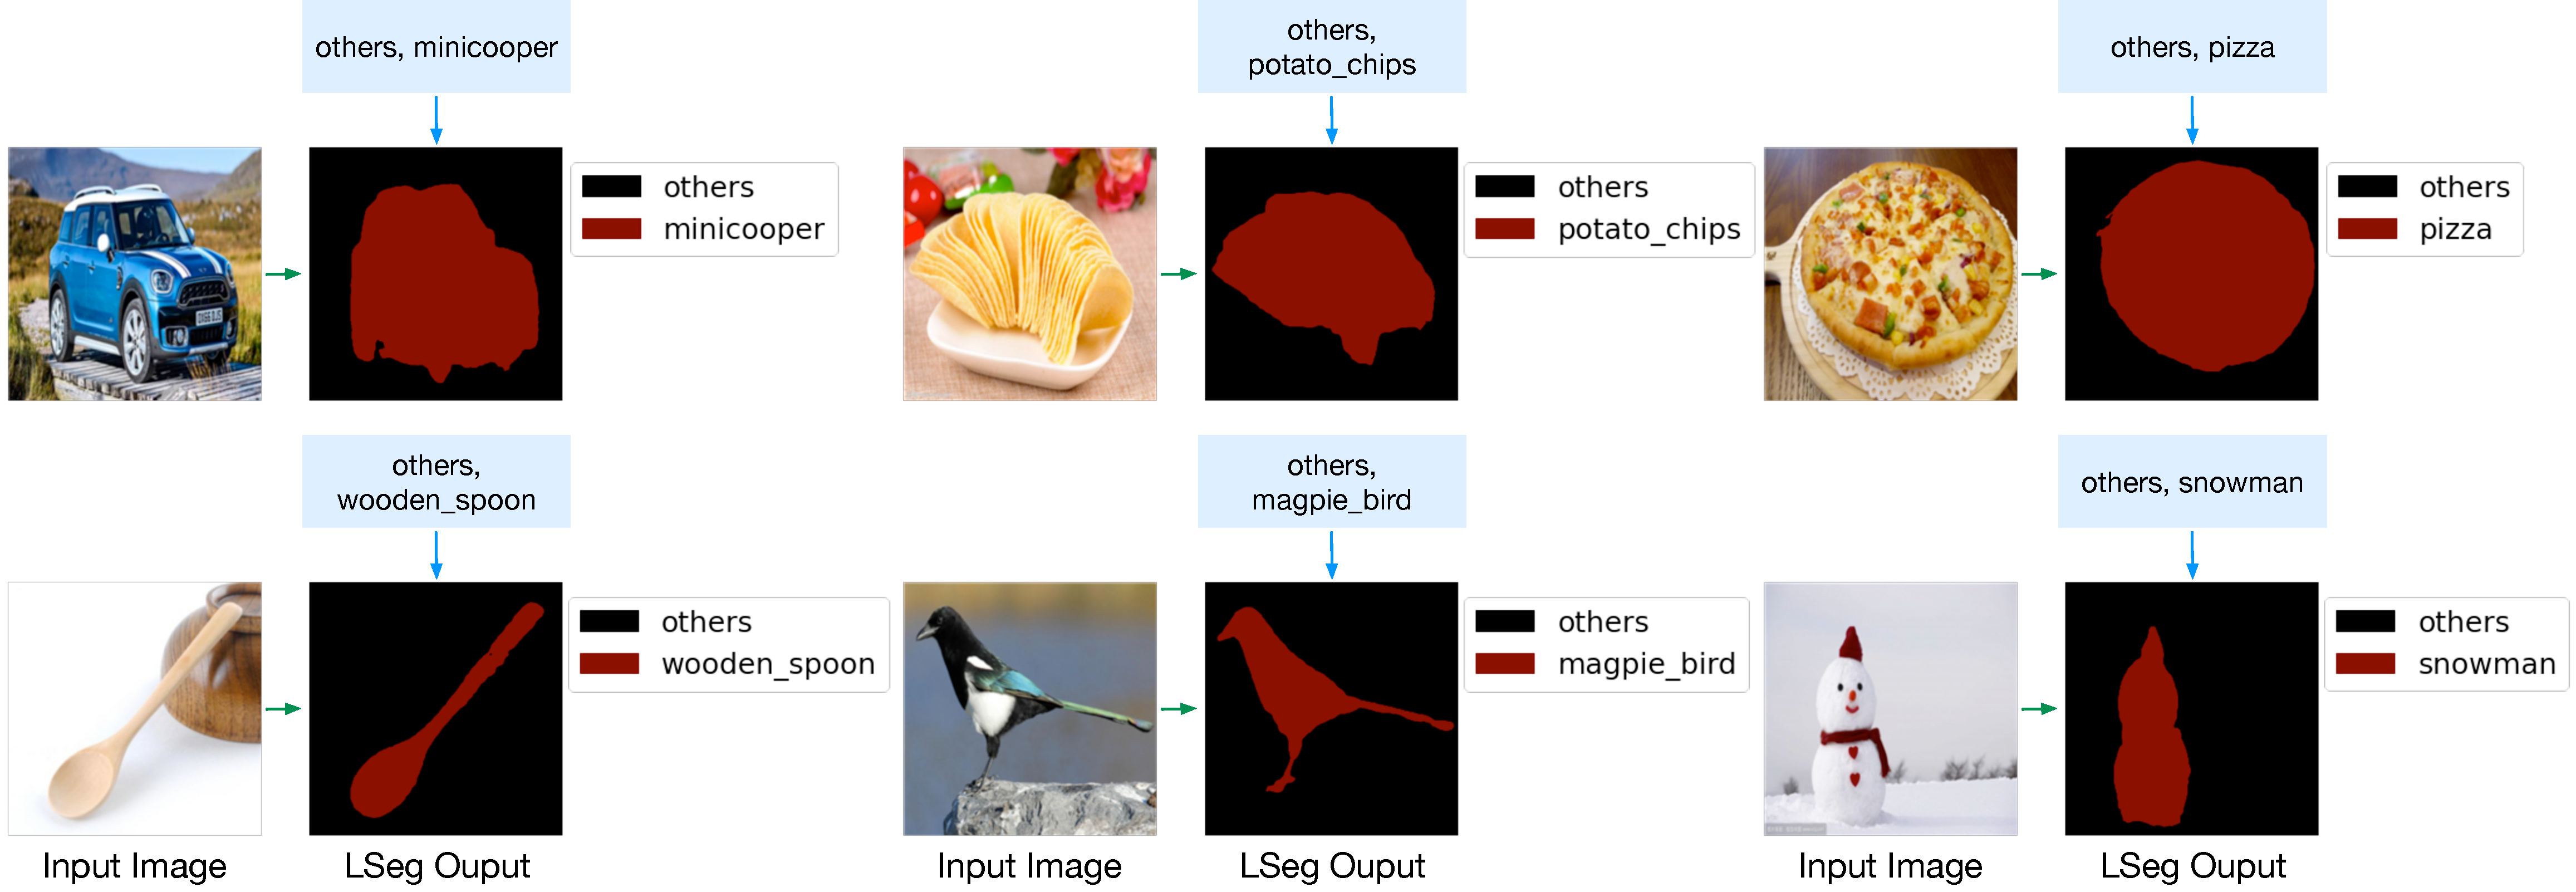
\includegraphics[width=\linewidth]{imgs/example_illustration1.pdf}
    \caption{\methodname{} zero-shot semantic segmentation results on unseen categories of FSS-1000 dataset.
    }
    \label{fig:example_illustration1}
\end{figure}
\vspace{-0.2in}







